\documentclass[a4paper]{article}
\usepackage[UTF8]{ctex}
\usepackage[left=3.17cm, right=3.17cm, top=2.54cm, bottom=2.54cm]{geometry}

\usepackage{fancyhdr}
\usepackage{graphicx, subfigure}
\usepackage{minted}
\setmonofont[]{Fira Code}
\usepackage[shortlabels]{enumitem}
\setenumerate{itemsep=0pt,partopsep=0pt,parsep=\parskip,topsep=0pt, itemindent=4em, leftmargin=0pt, listparindent=2em, label=(\arabic*)}
\setitemize{itemsep=0pt,partopsep=0pt,parsep=\parskip,topsep=5pt}
\setdescription{itemsep=0pt,partopsep=0pt,parsep=\parskip,topsep=5pt}

\usepackage[sort&compress]{gbt7714}
\usepackage{hyperref}
\hypersetup{unicode, colorlinks=true, linkcolor=black, urlcolor=black}
\usepackage{booktabs}
\usepackage{multirow}

\begin{document}

\definecolor{bg}{rgb}{0.95,0.95,0.95}

\title{\textbf{流水线MIPS处理器设计}\\——夏季学期综合实验报告}
\author{暮月}
\date{}
\maketitle

\tableofcontents

\newpage

\section{设计方案}

\subsection{总体设计}

使用Verilog,结合Vivado的IP Core生成的Distributed Memory,设计了支持MIPS核心指令子集的五级流水线。其总体设计图如图\ref{fig:总设计}。最终设计与设计图略有不同,但差异很小,主体结构与设计一致。

\begin{figure}[ht]
    \centering
    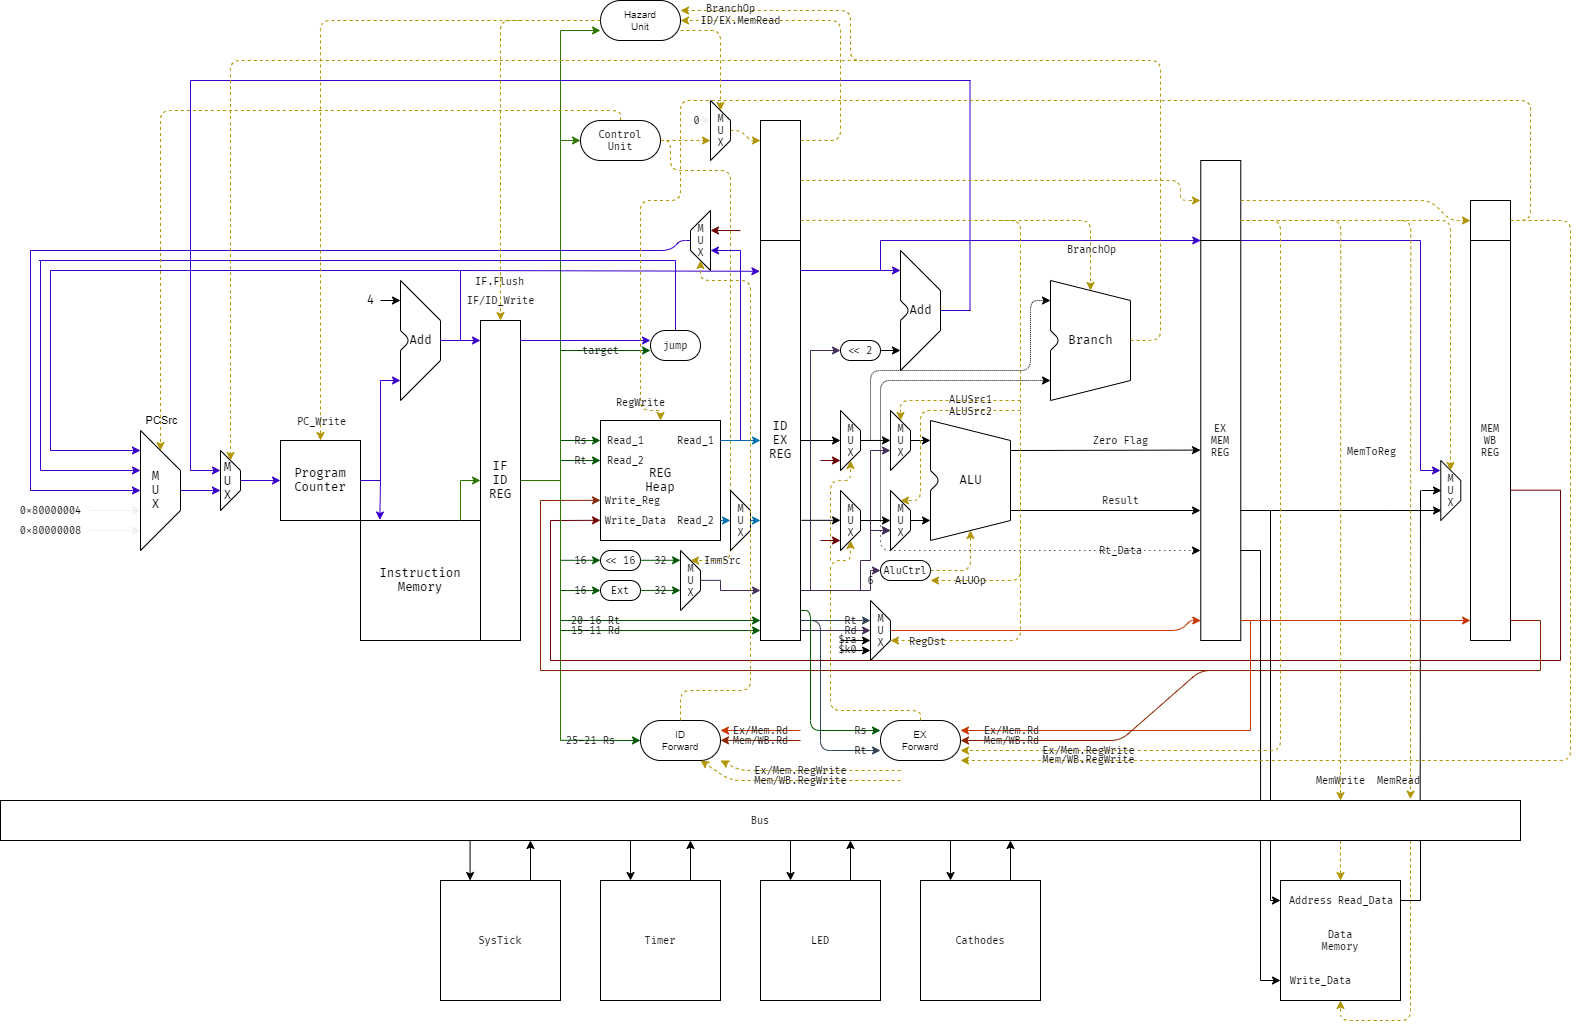
\includegraphics[width=.8\textwidth]{../assets/design.png}
    \caption{流水线总设计图}
    \label{fig:总设计}
\end{figure}

此CPU支持指令如表

\begin{table}[htb]
    \centering
    \caption{支持指令}
    \begin{tabular}{cc}
        \toprule
        类型 & 指令                                                                                     \\
        \midrule
        R型  & sll, srl, sra, jr, jalr, add, addu, sub, subu, and, or, xor, nor, slt, sltu              \\
        I型  & bltz, bgez, beq, bne, blez, bgtz, addi, addiu, slti, sltiu, andi, ori, xori, lui, lw, sw \\
        J型  & j, jal                                                                                   \\
        \bottomrule
    \end{tabular}
\end{table}

CPU为五级流水线的设计,即分为取指令(IF)、译指令(ID)、执行(EX)、访存(MEM)、写回(WB)五个阶段。后文均用缩写代称各阶段。

CPU有2048Bytes的指令存储器和数据存储器。

CPU仅支持处理最简单的“指令不支持”异常和由总线来的中断请求。采用完全的Forwarding解决数据依赖的冒险,并模拟寄存器堆的先写后读。对于Load-Use冒险,采取stall一周期的方式进行解决。

分支指令在EX阶段进行跳转,J型指令与jr和jalr在ID阶段进行跳转。jr和jalr前一条指令如果写入目标寄存器,需要在汇编层面插入nop指令以保证跳转位置正确。下面逐项介绍此CPU的设计细节。

\subsection{IF阶段}

IF阶段进行PC的更新和指令存储器的访问。PC采用Verilog代码编写的上升沿触发寄存器,指令存储器为使用Vivado的Distributed Memory Generator生成的ROM。使用这种ROM的好处是可以使用COE文件对其中数据进行初始化,实验中的汇编代码均使用Mars模拟器转为16进制后放入COE文件,再使用Vivado对指令存储器进行初始化,之后再进行综合与实现。

\begin{figure}[htb]
    \centering
    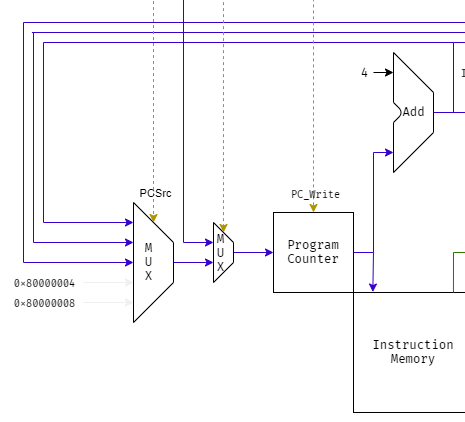
\includegraphics[width=.5\textwidth]{../assets/design_IF.png}
    \caption{IF阶段设计图}
    \label{fig:IF_design}
\end{figure}

IF阶段设计图如图\ref{fig:IF_design}。当时钟上升沿到来时,PC会根据控制信号进行更新,更改为PC+4、jump\_target、jr\_target、branch\_target、0x80000004、0x80000008中的一个,分别对应顺序执行、跳转和分支的目标、中断、异常。指令存储器为ROM,无时钟控制,根据输入地址输出对应指令。

PC的写入受控制信号PC\_Write的控制,具体细节见节\ref{sec:branchjump}。写入的中断和异常对应的控制信号细节见节\ref{sec:intexc}。

\subsection{ID阶段}

ID阶段将IF阶段取出的指令进行译码,并访问寄存器堆取值。此阶段还进行立即数的扩展、控制信号的生成、冒险的判断、跳转目标的生成、ID阶段的转发。其设计图如\ref{fig:ID_design}。

\begin{figure}[htb]
    \centering
    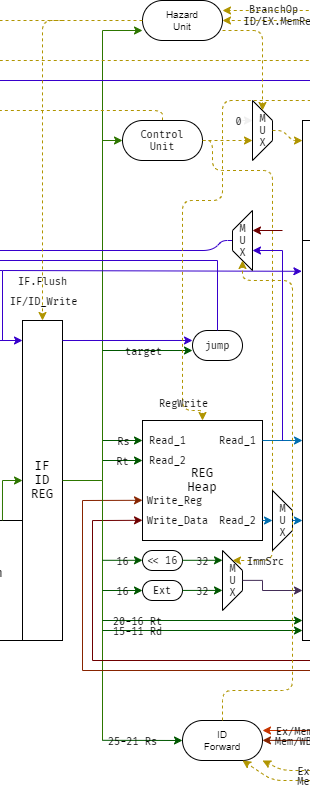
\includegraphics[width=.25\textwidth]{../assets/design_ID.png}
    \caption{ID阶段设计图}
    \label{fig:ID_design}
\end{figure}

IF和ID间为上升沿触发的流水线寄存器IF\_ID\_Reg,存储IF阶段取出的指令和PC+4。

寄存器堆为Verilog代码实现的类似RAM的结构,读取寄存器为组合逻辑,写寄存器需时钟和MEM\_WB\_Reg中存储的RegWrite信号一起触发。采用ID\_Forward对寄存器取值进行转发,模拟先写后读的功能。注意,这里设计图的转发有一定错误。寄存器的两个输出都进行转发,其中Read\_1的输出数据进行转发后再作为jr的目标地址和下一阶段的输入数据。其结构与对Read\_2的转发类似,但由于设计图已基本绘制完毕,不方便更改而遗留了这一处错误。

立即数扩展部分进行三种扩展方式:左移16位、符号扩展、零扩展,采用控制信号ExtOp和ImmSrc进行控制。

控制信号产生模块接收指令的OpCode和Funct,以及中断请求IRQ和监督信号Supervised,产生CPU绝大部分的控制信号。部分控制信号写入流水线寄存器,部分直接连接到其他模块进行控制。

冒险模块和转发模块的细节见节\ref{sec:hazard}。

\subsection{EX阶段}

EX阶段主要使用ALU进行整型运算,同时生成分支目标和branch\_hazard信号。其设计图如\ref{fig:EX_design}。

\begin{figure}[htb]
    \centering
    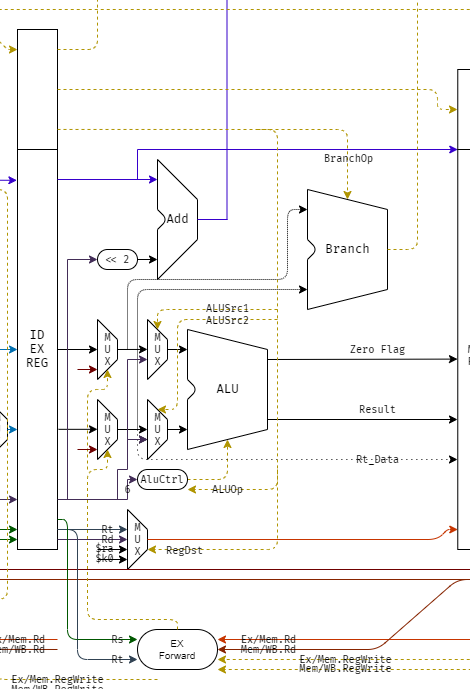
\includegraphics[width=.3\textwidth]{../assets/design_EX.png}
    \caption{EX阶段设计图}
    \label{fig:EX_design}
\end{figure}

ALU接收两个32位整型数据,支持位运算(与、或、异或、或非、左移、逻辑右移、代数右移)、加法、减法、小于比较功能。其控制信号由ALUControl接收ID\_EX\_Reg存储的控制信号后产生。

Branch接收两个32位整型数据,根据控制信号进行等于、不等于、小于等于零、大于等于零、小于零、大于零的判断。其输出为branch\_hazard信号,即为高电平时需要进行分支跳转。同时,将ID\_EX\_Reg存储的立即数左移两位后,与存储的PC+4求和,得到分支目标。

来自ID\_EX\_Reg的寄存器堆读出数据进行EX阶段的转发,然后与立即数一起接收控制信号的选择,由指令功能决定是否输入ALU。其转发细节见节\ref{sec:hazard}。

EX阶段还根据控制信号,在Rt、Rd、\$ra、\$k0中选择一个作为该指令的写入寄存器。

\subsection{MEM阶段}

MEM阶段对数据存储器进行访存。由于此CPU设计中需要加入外设,故设计了总线,并将外设和数据存储器作为其子模块。故对于CPU,此阶段为与总线的交互。MEM阶段的设计图见\ref{fig:MEM_design},总线的设计图见\ref{fig:Bus_design}。

\begin{figure}[htb]
    \centering
    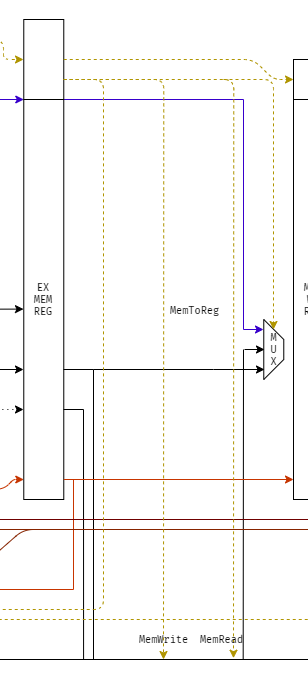
\includegraphics[width=.3\textwidth]{../assets/design_MEM.png}
    \caption{MEM阶段设计图}
    \label{fig:MEM_design}
\end{figure}

\begin{figure}[htb]
    \centering
    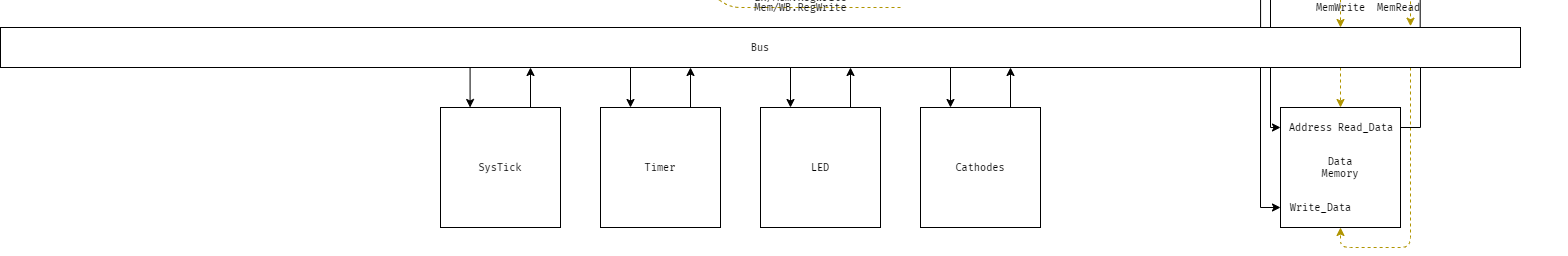
\includegraphics[width=.9\textwidth]{../assets/design_Bus.png}
    \caption{Bus设计图}
    \label{fig:Bus_design}
\end{figure}

对于抽象出来的总线,CPU在此阶段有控制信号读使能、写使能,以及32位地址、输入、输出。由于有中断请求和输出到数码管与LED的需要,CPU接收来自总线的相关信号。在时钟上升沿,如果读使能,总线输出地址对应的数据;如果写使能,将相应数据写入。由于此处理器一个周期只能执行写或者读,故32位地址共享,不作区分。

具体各外设和数据存储器的实现见节\ref{sec:bus}。

MEM阶段还根据EX\_MEM\_Reg中存储的MemToReg信号,从PC、PC+4、Rt内容、访存结果中选择写入寄存器堆的数据。

\subsection{WB阶段}

本阶段不产生任何信号,仅在时钟上升沿根据控制信号决定是否写入寄存器堆。为了模拟先写后读,本阶段的写入数据会参入其他阶段的转发。

由于寄存器堆的写入位上升沿触发,且与流水线寄存器为同一时钟控制,实际写入会晚一周期。不过由于采用转发机制,对汇编程序的执行没有影响。

\subsection{分支与跳转\label{sec:branchjump}}

CPU支持j、jal、jr、jalr以及多条分支指令,分别在ID阶段和EX阶段进行判断和执行。

对于j、jal、jr、jalr四条指令,在ID阶段控制信号产生模块生成jump\_hazard信号,传入冒险处理模块。冒险处理模块产生IF\_Flush信号,将IF\_ID\_Reg的指令置为32位0,从而清理掉下一个周期ID阶段将译码的信号。

由于jr和jalr需要访问寄存器Rs,故使用转发将前前条和前前前条指令对应要写入的指令转发。而对于前一条指令,可以采用类似Load-Use冒险判断的方式,进而延迟一个周期。但由于连线较多,改为汇编程序中添加一个nop指令的方式进行解决。即需要采用类似下方的语句以保证跳转结果的正确性。

\begin{minted}[bgcolor=bg]{matlab}
    to_user_mode:
    la      $ra, main
    nop
    jr      $ra
\end{minted}

对于分支指令,处理器默认不跳转,即IF和ID不暂停工作。在分支指令的ID阶段,控制信号产生模块根据分支指令的类型,产生BranchOp并存储到流水线寄存器中。在EX阶段,Branch模块接收转发后的rs\_data和rt\_data作为输入,并进行相关判断。当判断为真时,branch\_hazard信号拉高,冒险模块随即产生IF\_Flush和ID\_Flush指令,将对应的IF\_ID\_Reg和ID\_EX\_Reg中的关键信号改为0,即清理掉错误的指令。而当判断为假时,处理器继续运行,可以减少一定的CPI。简言之,此CPU对分支的预测总为假。

PC的更新会先根据PCSrc在PC+4、跳转目标、异常和中断处理地址中进行选择,再根据branch\_hazard决定是否跳转去分支目标。这个设计是有一定缺陷的,错误地将分支的优先级置于异常和中断之上,在特殊情况下会出现错误,应进行修改。

\subsection{冒险的应对\label{sec:hazard}}

MIPS流水线处理器中主要有三类冒险:结构冒险、数据冒险和控制冒险。在节\ref{sec:branchjump}中已经介绍了处理控制冒险的Flush信号,而此处理器各部分一周期只进行一项工作,不存在结构冒险。下面介绍数据冒险的应对。

\begin{figure}[htb]
    \centering
    
\includegraphics[width=.8\textwidth]{../assets/hazard.png}
    \caption{数据冒险处理示意图}
    \label{fig:hazard}
\end{figure}

数据冒险表现为当前指令需要寄存器Rs和Rt中的数据,而前面的三条指令的写入寄存器Rd可能恰好是这两个寄存器。此CPU采用转发以解决此问题。下面阐述图\ref{fig:hazard}中的四条转发路径的设计思路和其解决的问题。

\begin{enumerate}[1)]
    \item MEM\_WB转发到ID

          由于寄存器堆和流水线寄存器使用了同一时钟进行控制,实际写寄存器在WB阶段之后的一个周期开始时。将MEM\_WB\_Reg中的write\_data转发到ID,模拟了先写后读,保证WB阶段的同时的ID可以拿到要写入的值。

          对于这一问题,也可以将写入寄存器的操作提前到MEM进行,即MEM准备好写使能信号和数据,在WB开始时便可以直接写入寄存器堆,使用组合逻辑的读端口也能拿到数据。不过涉及改动较大,此CPU未采用这种策略。

    \item EX\_MEM转发到ID

          对于前前条执行写入寄存器的指令,不可能从寄存器中读取数据。而jr和jalr指令需要读取Rs寄存器的数值。故将EX阶段的结果从EX\_MEM\_Reg转发到ID阶段,从而不需要添加nop指令或者stall便可以在ID阶段进行跳转。

    \item MEM\_WB转发到EX

          对于前前条、执行访存或者其他需要写入寄存器的指令,可以采取从MEM\_WB\_Reg转发到EX阶段的策略,将同一时刻正在WB阶段的写入数据用于EX的计算功能中。

    \item EX\_MEM转发到EX

          对于前一条、需要写入寄存器的指令,可以采取从EX\_MEM\_Reg转发到EX阶段的策略,将同一时刻正在MEM阶段的写入数据用于EX的计算功能中。
\end{enumerate}

此外还有Load-Use这种特殊的数据冒险,即访存指令后紧接着要使用访存得到的数据这一冒险。由于访存发生在MEM阶段,无法直接转发到ID或者EX阶段。故需要先stall一个周期,再将MEM\_WB\_Reg中存储的数据转发到EX,从而解决这一冒险。stall的具体实现为将PC和的IF\_ID\_Reg写使能信号拉低,从而让PC和IF\_ID\_Reg暂停更新一个周期。

与之类似,jr和jalr前如果向对应寄存器写数据,同样会导致使用数据时还未写入正确的数据。可以增加电路实现类似的stall机制,但涉及改动较多,CPU未实现此机制。需要在汇编代码中添加nop指令。

\subsection{中断与异常\label{sec:intexc}}

此CPU支持最简单的“指令不支持”异常。其实现逻辑为在ID阶段的控制信号生成时根据OpCode和Funct判断是否为已实现指令,如果不是且当前不是内核态,则置Exception为1。相关的PCSrc、BranchOp等信号也根据Exception信号进行变化,保证此时准确的跳转到0x80000008。

中断的处理与异常类似,当外部中断请求进入控制信号生成单元后,调整控制信号,让PC准确地更改为0x80000004。

更加具体地,当异常或中断触发时,控制信号生成单元将PCSrc改为011或100,对应0x80000004和0x80000008两个地址;将BranchOp改为0,即禁止分支跳转功能;将RegWrite置为1,将RegDst置为11(对应选择\$k0),即将发生异常或者中断的地址写入寄存器(\$k0);将MemToReg置为10,对应选择PC+4作为写入寄存器数据的来源。

在控制信号发生变化后,PCSrc阻止冒险模块将IF\_Flush信号拉高,确保PC可以顺利更改为中断和异常处理程序的入口地址0x80000004和0x80000008。

当进入异常和中断的处理程序后,PC最高位为1,对应内核态。为保证内核态的监督信号在中断和异常处理时准确的一直为高,监督信号为PC和IF\_ID\_Reg中的PC+4最高位的或。当监督信号被拉高后,控制信号生成单元中保持Exception为0,同时也不接受外部中断请求,直到相应的处理程序通过jr或者jalr将PC最高位置为0,监督信号被拉低。

在此CPU的设计中,中断请求只来自总线的IRQ信号。

\subsection{总线与外设\label{sec:bus}}

此CPU的数据存储器和其他外设一齐被抽象为总线的子模块,CPU访存阶段仅直接和总线交互,由总线将数据根据地址转接到各个外设。下面逐个介绍各外设。

\subsubsection{数据存储器}

数据存储器与指令存储器类似,为使用Vivado的Distributed Memory Generator生成单口RAM。其使用一个时钟的上升沿和一个写使能信号控制写入,而读取数据为组合逻辑。使用Vivado生成这样一个RAM的好处在于使用COE文件对其进行初始化,减少了仿真的麻烦。对于实际上板应用,应考虑添加串口对数据存储器中数据进行初始化。

数据存储器的使用与寄存器堆基本一致,即读没有延迟,而写会因为流水线寄存器和总线传递给数据存储器的时钟一致,导致晚一个周期。然而一般MIPS的汇编代码中基本不可能出现先存数据再读同一地址的行为,故此问题应可以忽略。

\subsubsection{LED}

LED接受一个32位的输入,在时钟上升沿且写使能时将输入存储到寄存器中。当复位信号使能时,LED的寄存器会清空。

由于此CPU的设计目标为运行在指定的FPGA板上,LED数量有限,故仅将LED寄存器的低八位接出,作为总线的输出信号,进而连接到CPU的最外层输出,绑定在板卡的相应管脚上。

\subsubsection{七段数码管(SSDT)}

七段数码管(seven segment digital tube, SSDT)接收一个32位的输入,在时钟上升沿且写使能时将其低12位存入寄存器中。

在复位信号使能时,寄存器值置为FFFF\_FFFF\_FFFF。最高4位为数码管位选信号,低8位为数码管段选信号,高电平点亮。

由于此外设并不进行译码,需要汇编指令译码。参照汇编指令的switch可以使用下方指令进行译码(待译码四位信号存于\$t2,位选信号存于\$t0,部分指令已省略):

\begin{minted}[bgcolor=bg]{matlab}
BCD_switch:
    la      $t1, BCD
    lui     $t3, 0x8000
    sll     $t4, $t2, 2
    add     $t4, $t4, $t1
    add     $t4, $t4, $t3
    nop
    jr      $t4

BCD:
    j       bcd_0
    j       bcd_1
...

bcd_0:
    li      $t1, 0x3F
    add     $t0, $t0, $t1
    j       interruptExit
...
\end{minted}

此代码可以根据待译码的数字大小跳转到对应的\mintinline{matlab}{j bcd_X},进而跳转到对应的信号合成部分,得到正确的12位控制信号。将这个信号存入SSDT后即可正确点亮。

\subsubsection{系统时钟计数器(SysTick)}

SysTick为一个计数器,时钟上升沿时加一,不能写。当总线读使能时,可以取出其计数的值。

\subsubsection{定时器}

定时器有3个32位寄存器,分别成为TH、TL、TCON,因而占据总线上的连续12字节空间。当TCON最低位的计时使能为1时,TL不断增加直到变为0xFFFFFFFF,然后变为TH后再次自增。同时如果TCON的第2位允许中断为1,则TCON的第3位被拉高,视为对CPU的中断请求,输出到总线的IRQ,其后CPU的行为见节\ref{sec:intexc}。

\section{关键代码与文件清单}

\subsection{文件清单}

源代码均位于src文件夹中,其中ip文件夹下的dist\_mem\_gen\_ins和dist\_mem\_gen\_data为Vivado的IP Core生成文件。

\begin{minted}[bgcolor=bg]{matlab}
    src
    ├─configs
    │      cpu.xdc              约束文件
    ├─designs
    │  │  ALU.v                 ALU
    │  │  ALUControl.v          ALU控制信号生成单元
    │  │  Branch.v              分支判断
    │  │  Bus.v                 总线
    │  │  Control.v             控制信号生成单元
    │  │  CPU.v                 CPU 顶层文件
    │  │  DataMem.v             数据存储器
    │  │  EX_Forward.v          EX阶段转发控制
    │  │  EX_MEM_Reg.v          EX MEM 间流水线寄存器
    │  │  Hazard.v              冒险单元
    │  │  ID_EX_Reg.v           ID EX 间流水线寄存器
    │  │  ID_Forward.v          ID阶段转发控制
    │  │  IF_ID_Reg.v           IF ID 间流水线寄存器
    │  │  InstructionMem.v      指令存储器
    │  │  MEM_WB_Reg.v          MEM WB 间流水线寄存器
    │  │  ProgramCounter.v      PC寄存器
    │  │  Register.v            寄存器堆
    │  ├─ip
    │  │  ├─dist_mem_gen_data   数据存储器核心
    │  │  └─dist_mem_gen_ins    指令存储器核心
    │  ├─ip_init
    │  │      data_init.coe     数据存储器初始化文件
    │  │      ins_init.coe      指令存储器初始化文件
    │  └─peripherals
    │          LED.v            LED
    │          SSDT.v           七段数码管
    │          SysTick.v        系统时钟计数器
    │          Timer.v          定时器
    └─tests
        │  tb_CPU.v             CPU testbench
        │  tb_InstructionMem.v  ins_mem testbench
        └─asm
                a.in                    Mars测试用读入文件
                a.out                   Mars测试用输出文件
                bubble_sort.asm         冒泡排序汇编
                bubble_sort.hex         冒泡排序汇编16进制码
                bubble_sort_Mars.asm    Mars测试用冒泡排序汇编
                gen.py                  a.in生成用py
\end{minted}

\subsection{关键代码}

CPU.v PC更新代码

\begin{minted}[bgcolor=bg]{verilog}
assign PC_p4 = {PC[31], PC[30: 0] + 31'd4};
assign PC_next =
       branch_hazard ? branch_target :
       (PCSrc == 3'b000) ? PC_p4 :
       (PCSrc == 3'b001) ? jump_target :
       (PCSrc == 3'b010) ? jr_target :
       (PCSrc == 3'b011) ? 32'h80000004 :
       (PCSrc == 3'b100) ? 32'h80000008 :
       32'h80000000;
ProgramCounter program_counter(
                 .clk(clk),
                 .reset(reset),
                 .wen(PC_wen),
                 .pc_next(PC_next),
                 .pc(PC)
               );
\end{minted}

CPU.v ID阶段转发

\begin{minted}[bgcolor=bg]{verilog}
assign rs_data_forward_id =
    (id_forward_1 == 2'b00) ? rs_data :
    (id_forward_1 == 2'b01) ? ex_mem.alu_out :
    mem_wb.write_data;
assign rt_data_forward_id = id_forward_2 ?
        mem_wb.write_data :
        rt_data;

\end{minted}

CPU.v EX阶段转发及ALU输入控制

\begin{minted}[bgcolor=bg]{verilog}
assign rs_data_forward_ex =
    (ex_forward_1 == 2'b01) ? ex_mem.alu_out :
    (ex_forward_1 == 2'b10) ? mem_wb.write_data :
    id_ex.rs_data;
assign rt_data_forward_ex =
    (ex_forward_2 == 2'b01) ? ex_mem.alu_out :
    (ex_forward_2 == 2'b10) ? mem_wb.write_data :
    id_ex.rt_data;

assign alu_src1 =
    (id_ex.ALUSrc[1 : 0] == 2'b01) ? id_ex.Imm :
    (id_ex.ALUSrc[1 : 0] == 2'b10) ? 32'h0 :
    rs_data_forward_ex;
assign alu_src2 = id_ex.ALUSrc[2] ? 
        id_ex.Imm :
        rt_data_forward_ex;
\end{minted}

CPU.v 写回数据选择

\begin{minted}[bgcolor=bg]{verilog}
assign write_data =
    (ex_mem.MemToReg == 2'b10) ?
    (ex_mem.Rd == 5'd26 ?
     ex_mem.PC_p4 - 32'h4 :
     ex_mem.PC_p4) :
    (ex_mem.MemToReg == 2'b01) ? mem_out :
    ex_mem.alu_out;
\end{minted}

Hazard.v 冒险控制信号

\begin{minted}[bgcolor=bg]{verilog}
assign load_use_hazard =
    reset ? 1'b0 :
    ID_EX_MemRead &&
    (ID_EX_Rt == IF_ID_Rs ||
     ID_EX_Rt == IF_ID_Rt);

assign PC_wen = ~load_use_hazard;
assign IF_wen = ~load_use_hazard;

assign IF_Flush = 
    reset ? 
    1'b0 : 
    (jump_hazard || 
    branch_hazard) && 
    (PCSrc != 3'b011 && 
    PCSrc != 3'b100);
assign ID_Flush = reset ? 1'b0 : branch_hazard;
\end{minted}

Bus.v 总线与外设使能信号

\begin{minted}[bgcolor=bg]{verilog}
assign Data_Mem_en = (Address <32'h40000000) && en;
assign Data_Mem_wen = (Address <32'h40000000) && wen;

assign Timer_en = 
    (Address >= 32'h40000000 && 
    Address <= 32'h4000000B) ? 
    en : 0;
assign Timer_wen = 
    (Address >= 32'h40000000 &&
    Address <= 32'h4000000B) ? 
    wen : 0;

assign LED_en = (Address == 32'h4000000C) &&en;
assign LED_wen = (Address == 32'h4000000C) & wen;

assign SysTick_en = (Address ==32'h40000014) && en;

assign SSDT_en = (Address == 32'h40000010) & en;
assign SSDT_wen = (Address == 32'h40000010) & wen;

assign led = LED_dout[7 : 0];

assign dout =
       Data_Mem_en ? Data_Mem_dout :
       Timer_en ? Timer_dout :
       SysTick_en ? SysTick_dout :
       LED_en ? LED_dout :
       SSDT_en ? {20'b0, ssdt} : 32'h0;
\end{minted}

\section{综合与实现情况}

\subsection{资源使用与时序性能}

调整Vivado的flatten\_hierarchy为none、rebuild、full三种情况,针对100MHz时钟进行综合和实现,得到性能概览如图\ref{fig:综合实现性能概览}。

\begin{figure}[htb]
    \centering
    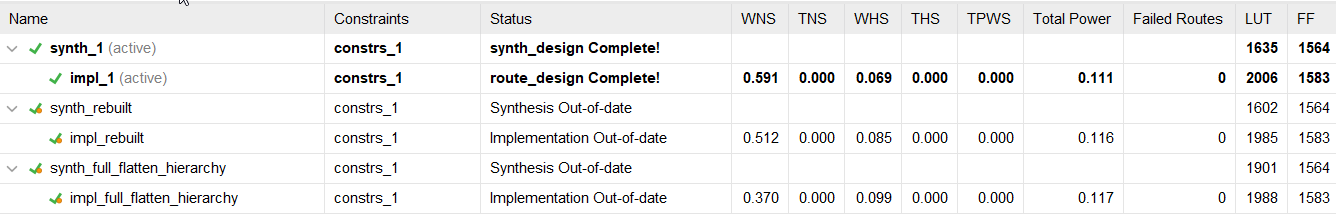
\includegraphics[width=.9\textwidth]{../assets/综合实现情况.png}
    \caption{综合实现性能概览}
    \label{fig:综合实现性能概览}
\end{figure}

总体上,不打平层次的时序裕量最多,达到0.591ns,但使用的LUT也最多,综合使用了1635个LUT和1564个触发器,实现后上涨到2006个LUT和1583个触发器。相比之下,rebuild和full两种模式进行层次打平后时序裕量下降,使用板上资源也没有较大的减幅,故下面针对不打平的情况进行分析。

逻辑使用情况见表\ref{tab:slice logic}。总体上实现使用了近10\%的LUT资源和近4\%的寄存器资源。一个较为复杂的MIPS5级流水线处理器只需要不到10\%的资源,这体现出了FPGA的巨大潜力。

\begin{table}[htb]
    \centering
    \caption{逻辑资源使用情况}
    \label{tab:slice logic}
    \begin{tabular}{lllll}
        \toprule
        Site Type                     & Used & Fixed & Available & Util\% \\
        \midrule
        Slice LUTs                    & 2006 & 0     & 20800     & 9.64   \\
        \quad LUT as Logic            & 1750 & 0     & 20800     & 8.41   \\
        \quad LUT as Memory           & 256  & 0     & 9600      & 2.67   \\
        \qquad LUT as Distributed RAM & 256  & 0     &           &        \\
        \qquad LUT as Shift Register  & 0    & 0     &           &        \\
        Slice Registers               & 1583 & 0     & 41600     & 3.81   \\
        \quad Register as Flip Flop   & 1583 & 0     & 41600     & 3.81   \\
        \quad Register as Latch       & 0    & 0     & 41600     & 0.00   \\
        F7 Muxes                      & 384  & 0     & 16300     & 2.36   \\
        F8 Muxes                      & 64   & 0     & 8150      & 0.79   \\
        \bottomrule\end{tabular}
\end{table}

由于没有打平层次,可以进一步查看各层次使用的资源,使用情况见表\ref{tab:逻辑资源分层使用情况}。可以看到,使用资源最多的时寄存器堆,其次是总线和ALU。进一步优化板上资源应考虑减少这几处不必要的或者冗余的资源。

\begin{table}[H]
    \centering
    \caption{逻辑资源分层使用情况}
    \label{tab:逻辑资源分层使用情况}
    \begin{tabular}{llllllll}
        \toprule
        Name         & LUTs & Regs & F7 Mux & F8 Mux & Slice & LUT Logic & LUT Mem \\
        \midrule
        CPU          & 2006 & 1583 & 384    & 64     & 796   & 1750      & 256     \\
        (ALU)        & 406  & 0    & 0      & 0      & 111   & 406       & 0       \\
        (ALUControl) & 9    & 0    & 0      & 0      & 6     & 9         & 0       \\
        (Branch)     & 22   & 0    & 0      & 0      & 12    & 22        & 0       \\
        (Bus)        & 448  & 192  & 128    & 64     & 162   & 192       & 256     \\
        (Control)    & 26   & 0    & 0      & 0      & 12    & 26        & 0       \\
        (EX Forward) & 14   & 0    & 0      & 0      & 6     & 14        & 0       \\
        (EX MEM)     & 0    & 106  & 0      & 0      & 69    & 0         & 0       \\
        (Hazard)     & 7    & 0    & 0      & 0      & 4     & 7         & 0       \\
        (ID EX)      & 2    & 160  & 0      & 0      & 69    & 2         & 0       \\
        (ID Forward) & 10   & 0    & 0      & 0      & 3     & 10        & 0       \\
        (IF ID)      & 1    & 63   & 0      & 0      & 29    & 1         & 0       \\
        (InsMem)     & 110  & 0    & 0      & 0      & 34    & 110       & 0       \\
        (MEM WB)     & 0    & 38   & 0      & 0      & 26    & 0         & 0       \\
        (PC)         & 0    & 32   & 0      & 0      & 8     & 0         & 0       \\
        (Register)   & 607  & 992  & 256    & 0      & 418   & 607       & 0       \\
        \bottomrule
    \end{tabular}
\end{table}

\begin{figure}[H]
    \centering
    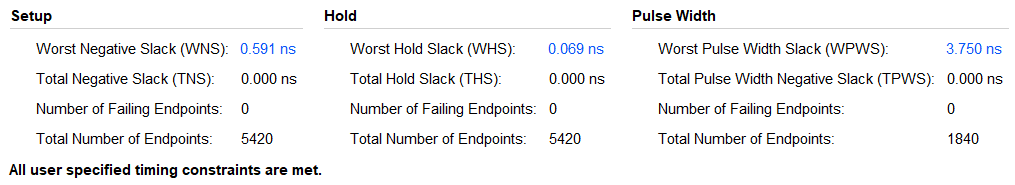
\includegraphics[width=.9\textwidth]{../assets/imp_none_flatten_timing.png}
    \caption{实现时序裕量}
    \label{fig:实现时序裕量}
\end{figure}

实现后的时序裕量为0.591ns,最长路径的电路见图\ref{fig:最长路径},细节见图\ref{fig:最长路径细节}。。可以看出,这一条路径是从MEM\_WB向EX阶段转发寄存器,进入分支判断模块后再进入冒险单元产生IF\_Flush信号。这表明此处理器的控制信号产生较为复杂,需要多个模块逐级产生。也因为过于复杂,优化难度较大,经过尝试后我认为需要对总设计做出较大的改动,遂放弃。

\begin{figure}[H]
    \centering
    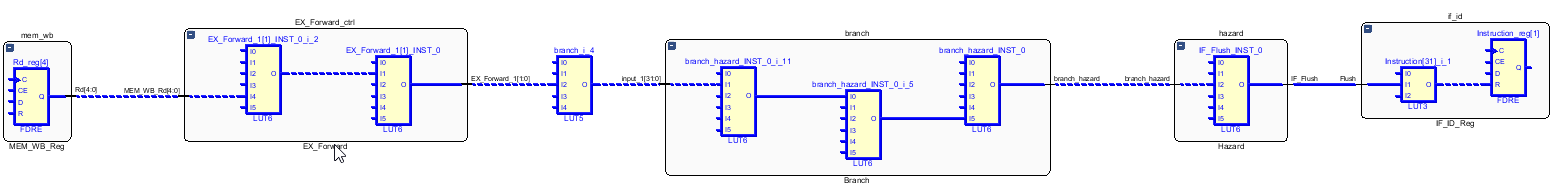
\includegraphics[width=.9\textwidth]{../assets/最长路径.png}
    \caption{最长路径}
    \label{fig:最长路径}
\end{figure}

\begin{figure}[H]
    \centering
    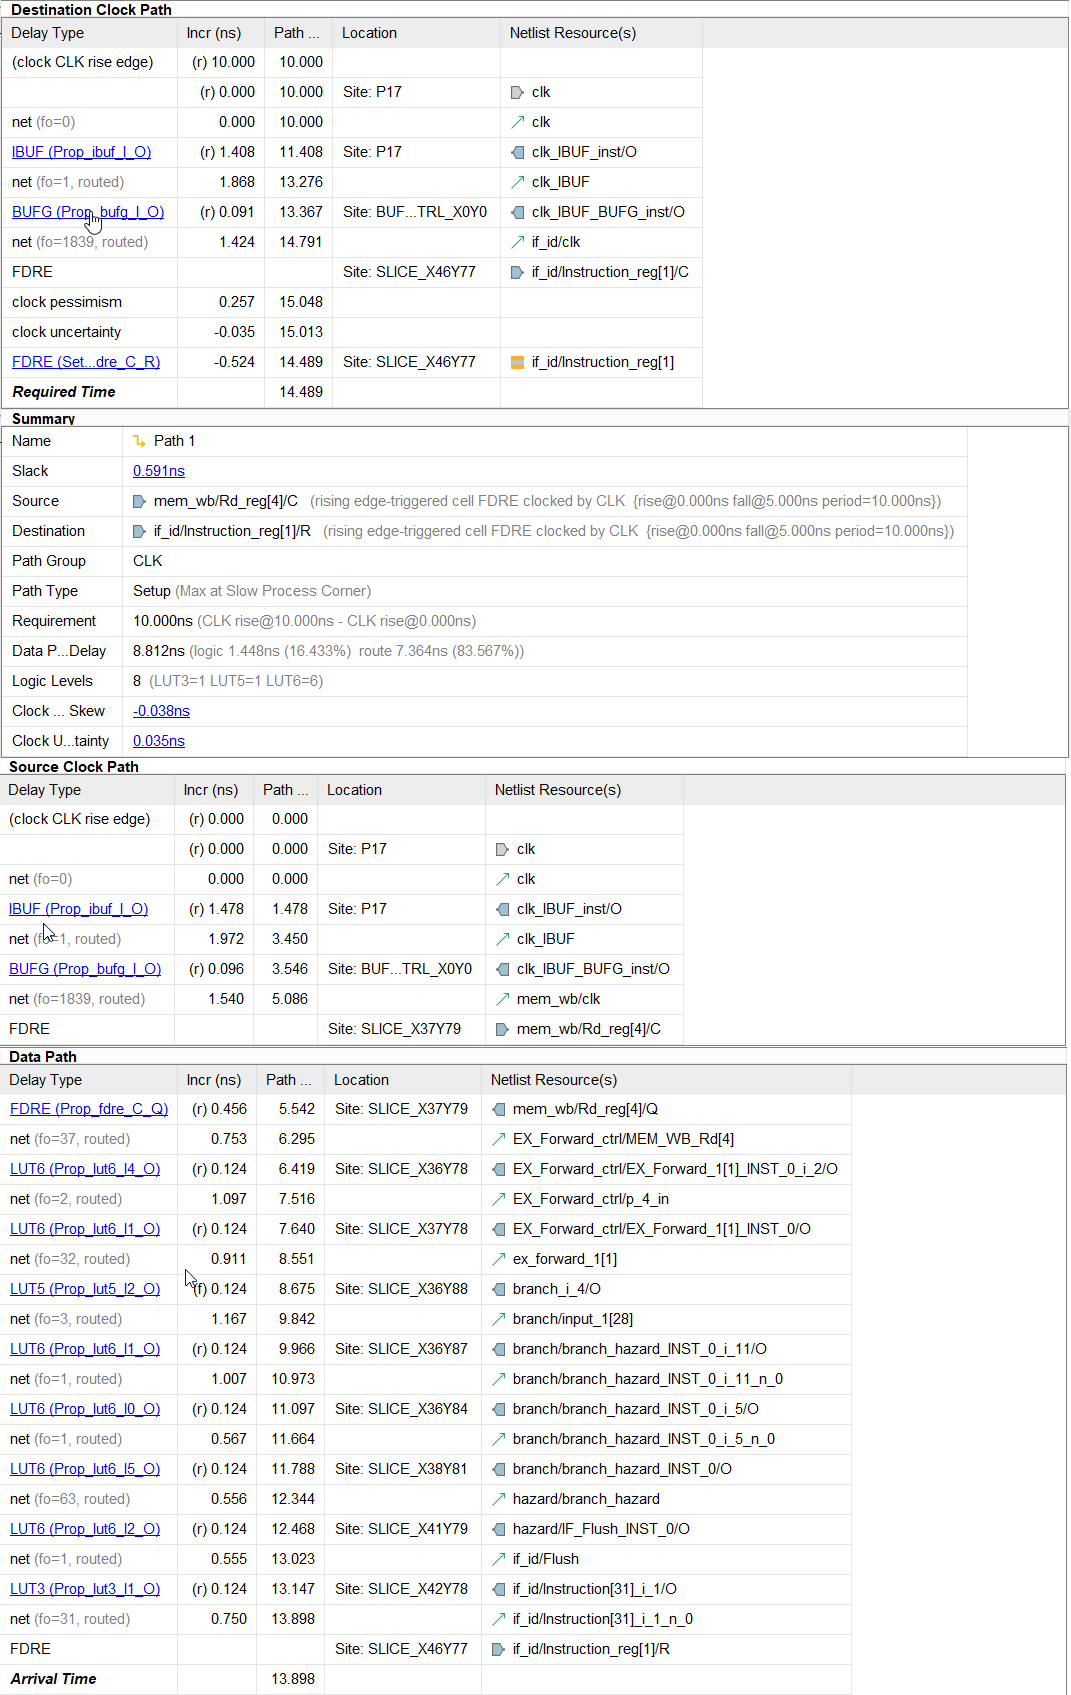
\includegraphics[width=.5\textwidth]{../assets/最长路径_细节.png}
    \caption{最长路径细节}
    \label{fig:最长路径细节}
\end{figure}

实现结果表明,此CPU的主频可以达到106.281MHz。

\subsection{仿真验证}

仿真验证分两部分:Vivado仿真与Mars验证。使用的汇编代码见附录\ref{adx:asm},其内容为使用冒泡排序对一组设计好的,放在数据存储器0-127行的数据进行排序。为节省仿真时间,排序用的数据如图\ref{fig:排序数据}。即只需将少数数字排序便全部有序。

\begin{figure}[H]
    \centering
    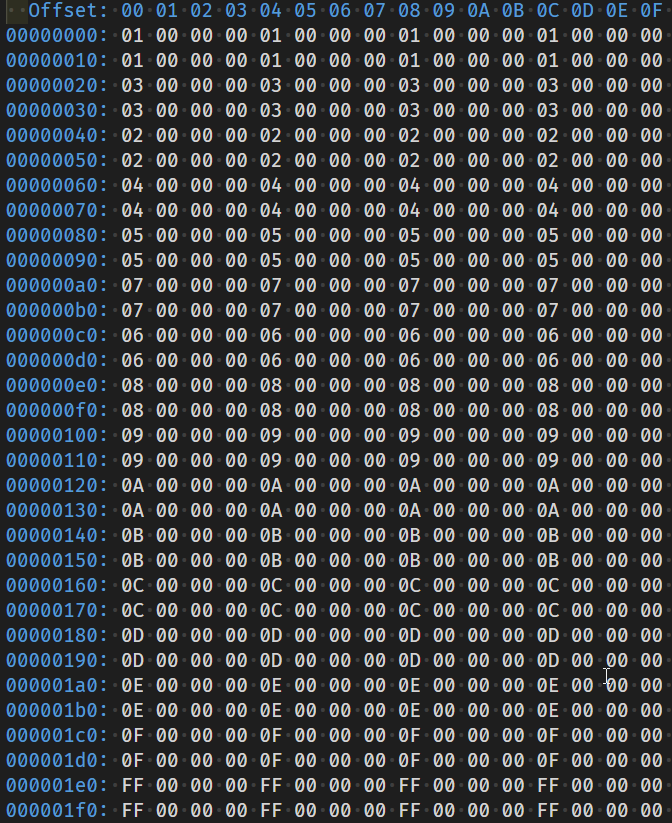
\includegraphics[width=.5\textwidth]{../assets/检验数据.png}
    \caption{排序数据}
    \label{fig:排序数据}
\end{figure}

由于没有进行层次打平,可以非常容易地查看寄存器中数据,下面查看仿真时用到的寄存器和最后输出的SSDT信号。

\begin{figure}[H]
    \centering
    \subfigure[排序开始寄存器数据]{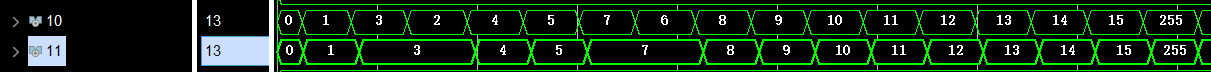
\includegraphics[width=.8\textwidth]{../assets/sorting.png}}
    \subfigure[排序结束寄存器数据]{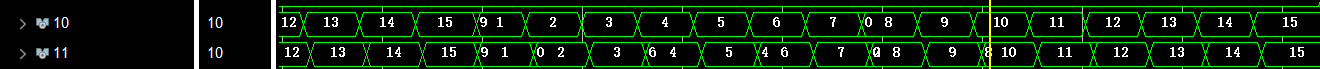
\includegraphics[width=.8\textwidth]{../assets/sorted_imp.png}}
    \subfigure[ssdt信号]{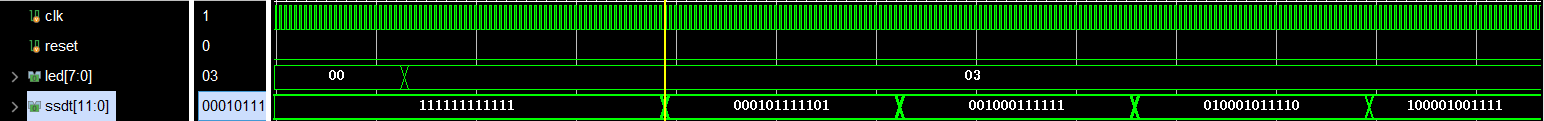
\includegraphics[width=.8\textwidth]{../assets/ssdt_imp.png}}
    \caption{仿真波形}
\end{figure}

可以看到,CPU顺利执行了冒泡排序,将设计好的数据进行了从小到大的排序,并且输出了周期“0x3D06",即执行了15622个周期。

使用脚本生成同样的数据的二进制文件,结合之前理论课汇编作业的代码和附录\ref{adx:asm}中的冒泡排序,用Mars模拟器统计排序过程中的指令数如图\ref{fig:指令数量}。得到总共指令数为11541,故CPI为1.3536。

\begin{figure}[H]
    \centering
    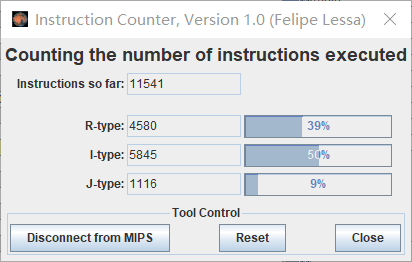
\includegraphics[width=.6\textwidth]{../assets/ins.png}
    \caption{指令数量}
    \label{fig:指令数量}
\end{figure}

由于此CPU的设计并未将分支跳转前移至ID阶段,且汇编代码并未特意按照分支发生的可能性进行编写,故CPI并不算很低。如果经过精心设计,CPI可能可以有较大的缩减。

综上,此CPU的主频为106.281MHz,测试用程序的CPI为1.3536。与单周期MIPS 32 CPU的66.1857MHz比起来有非常显著的提升。

\section{经验体会}

本次实验比较全面地体会了硬件设计的流程,学会了一些设计的思路。但是没有能够对设计进行比较好的优化,也未能尝试仿照《计算机组成与设计:硬件/软件接口》所叙述的超长指令字、超标量、分支预测等方法提高CPI,略有遗憾。

回顾本次实验,主要经验可以概括为下面两部分:

\begin{enumerate}
    \item \textbf{先设计,再实现,事半功倍}

          本次实验中,我先着手使用drawio绘制了CPU的总设计图,然后基于此设计图进行实现。因为在绘制设计图时已经思考了大部分信号的依赖关系,所以参照设计图使用Verilog进行实现节省了很多时间。但是由于时序电路设计经验不足,加之流水线处理器的细节处理知识还不够扎实,有些设计是不很正确甚至是整个设计的拖累。

          如果从头开始进行本实验,我认为我会在最初花更多的精力进行总设计,减少本次实验中设计完成后发现功能有问题而不断修修补补的方式。或许这样可以减少电路中的冗余部分,节省资源,优化时序性能。

    \item \textbf{利用好设计软件Vivado}

          在设计前,我咨询了几位学长使用Vivado进行硬件设计的经验。其中得到了两条对于本实验帮助很大的经验:“使用好IP Core”和“少用行为仿真,多用时序仿真”。

          基于前一条经验,我使用搜索引擎,结合Xilinx的Vivado使用指南,将单周期MIPS 32 CPU采用的组合逻辑指令存储器和人工编写的数据存储器换为Distributed Memory Generator生成的存储器。这样做最大的好处是方便修改代码和测试数据,节省了不少时间。

          最初我不太理解后一条经验,认为应该行为仿真没有问题再进行时序仿真。我实际进行实验后发现,行为仿真没有延时信息,与实际执行过程差异较大。为了保证CPU正常工作,直接进行综合实现后的时序仿真可以更快发现问题,并可以直接对着近乎实际的波形图进行分析,节省了大量时间。

          在实验的后半段,我基本上都是直接进行综合实现,然后针对有延时后的时序波形进行调整。这种调整比对着行为仿真的标准波形目测更加直观有效。

          此外,我还学会了配置仿真波形的显示窗口。在充分利用了Group和Divider后,波形窗口中不同阶段的信号很好地被区分开来,加快了寻找问题的速度。
\end{enumerate}

\nocite{syn}
\nocite{dmg}
\nocite{计算机组成与设计}

\small{
    \bibliographystyle{gbt7714-numerical}
    \bibliography{ref}
}

\newpage

\appendix

\section{仿真验证用汇编\label{adx:asm}}

\begin{minted}[bgcolor=bg]{matlab}
.text
    j   to_user_mode
    j   interrupt
    j   exception

to_user_mode:
    la  $ra,    main
    nop
    jr  $ra

main:
    # load SysTick => count clocks
    li      $s7, 0x40000000         # $s7 0x40000000
    lw      $s6, 20($s7)            # $s6 (0x40000014)

    # call bubble sort
    ori     $a0, $0, 0              # $a0 0x00000000 start addr
    ori     $a1, $0, 127            # $a1 n
    jal     bubble_sort

    # load SysTick
    lw      $s5, 20($s7)
    sub     $s4, $s5, $s6

    # lower 16 bits
    ori     $t0, $0, 0xF
    and     $s0, $t0, $s4
    srl     $s4, $s4, 4
    and     $s1, $t0, $s4
    srl     $s4, $s4, 4
    and     $s2, $t0, $s4
    srl     $s4, $s4, 4
    and     $s3, $t0, $s4

    # use led
    sw      $s4, 12($s7)

    ori     $s6, $0, 0

    # Timer interrupt
    subi    $t0, $0, 0x000F
    sw      $t0, 0($s7)             # TH = 0xFFFFFFF1
    subi    $t0, $0, 1
    sw      $t0, 4($s7)             # TL = 0xFFFFFFFF
    ori     $t0, $0, 3
    sw      $t0, 8($s7)

loop:
    j       loop

bubble_sort:
    addi    $sp, $sp, -12
    sw      $ra, 0($sp)
    sw      $s1, 4($sp)
    sw      $s0, 8($sp)

    move    $s0, $a0                # array addr
    move    $s1, $a1                # n

    move    $s2, $0                 # sorted = false

L0:
    bne     $s2, $0, L0end
    ori     $s2, 0x1

    li      $t0, 1
L1:
    bge     $t0, $s1, L1end

    sll     $t1, $t0, 2
    add     $t1, $t1, $s0
    lw      $t2, 0($t1)
    lw      $t3, -4($t1)
    ble     $t3, $t2, else
    sw      $t3, 0($t1)
    sw      $t2, -4($t1)
    move    $s2, $0
else:
    addi    $t0, $t0, 1
    j       L1
L1end:
    subi    $s1, $s1, 1
    j       L0
L0end:

    lw      $s0, 8($sp)
    lw      $s1, 4($sp)
    lw      $ra, 0($sp)
    addi    $sp, $sp, 12

    move    $v0, $0
    nop
    jr      $ra

interrupt:
    ori     $t0, $0, 1
    sw      $t0, 8($s7)

    la      $t1, show
    lui     $t2, 0x8000
    sll     $t0, $s6, 2
    add     $t0, $t0, $t1
    add     $t0, $t0, $t2
    nop
    jr      $t0

show:
    j       show_0
    j       show_1
    j       show_2
    j       show_3

show_0:
    li      $t0, 0x00000100
    move    $t2, $s0
    j       BCD_switch

show_1:
    li      $t0, 0x00000200
    move    $t2, $s1
    j       BCD_switch

show_2:
    li      $t0, 0x00000400
    move    $t2, $s2
    j       BCD_switch

show_3:
    li      $t0, 0x00000800
    move    $t2, $s3
    j       BCD_switch

BCD_switch:
    la      $t1, BCD
    lui     $t3, 0x8000
    sll     $t4, $t2, 2
    add     $t4, $t4, $t1
    add     $t4, $t4, $t3
    nop
    jr      $t4

BCD:
    j       bcd_0
    j       bcd_1
    j       bcd_2
    j       bcd_3
    j       bcd_4
    j       bcd_5
    j       bcd_6
    j       bcd_7
    j       bcd_8
    j       bcd_9
    j       bcd_A
    j       bcd_B
    j       bcd_C
    j       bcd_D
    j       bcd_E
    j       bcd_F

bcd_0:
    li      $t1, 0x3F
    add     $t0, $t0, $t1
    j       interruptExit
bcd_1:
    li      $t1, 0x6
    add     $t0, $t0, $t1
    j       interruptExit
bcd_2:
    li      $t1, 0x5B
    add     $t0, $t0, $t1
    j       interruptExit
bcd_3:
    li      $t1, 0x4F
    add     $t0, $t0, $t1
    j       interruptExit
bcd_4:
    li      $t1, 0x66
    add     $t0, $t0, $t1
    j       interruptExit
bcd_5:
    li      $t1, 0x6D
    add     $t0, $t0, $t1
    j       interruptExit
bcd_6:
    li      $t1, 0x7D
    add     $t0, $t0, $t1
    j       interruptExit
bcd_7:
    li      $t1, 0x7
    add     $t0, $t0, $t1
    j       interruptExit
bcd_8:
    li      $t1, 0x7F
    add     $t0, $t0, $t1
    j       interruptExit
bcd_9:
    li      $t1, 0x6F
    add     $t0, $t0, $t1
    j       interruptExit
bcd_A:
    li      $t1, 0x77
    add     $t0, $t0, $t1
    j       interruptExit
bcd_B:
    li      $t1, 0x7C
    add     $t0, $t0, $t1
    j       interruptExit
bcd_C:
    li      $t1, 0x39
    add     $t0, $t0, $t1
    j       interruptExit
bcd_D:
    li      $t1, 0x5E
    add     $t0, $t0, $t1
    j       interruptExit
bcd_E:
    li      $t1, 0x79
    add     $t0, $t0, $t1
    j       interruptExit
bcd_F:
    li      $t1, 0x71
    add     $t0, $t0, $t1
    j       interruptExit

interruptExit:
    addi    $s6, $s6, 1
    andi    $s6, $s6, 3

    sw      $t0, 16($s7)
    li      $t0, 3
    sw      $t0, 8($s7)            # TCon = 3
    jr      $k0

exception:
    j       exception


\end{minted}

\end{document}